\documentclass[journal,12pt,twocolumn]{IEEEtran}
\usepackage{setspace}
\usepackage{gensymb}
\usepackage{caption}
%\usepackage{multirow}
%\usepackage{multicolumn}
%\usepackage{subcaption}
%\doublespacing
\singlespacing
\usepackage{csvsimple}
\usepackage{amsmath}
\usepackage{multicol}
%\usepackage{enumerate}
\usepackage{amssymb}
%\usepackage{graphicx}
\usepackage{newfloat}
%\usepackage{syntax}
\usepackage{listings}
\usepackage{iithtlc}
\usepackage{color}
\usepackage{tikz}
\usetikzlibrary{shapes,arrows}



%\usepackage{graphicx}
%\usepackage{amssymb}
%\usepackage{relsize}
%\usepackage[cmex10]{amsmath}
%\usepackage{mathtools}
%\usepackage{amsthm}
%\interdisplaylinepenalty=2500
%\savesymbol{iint}
%\usepackage{txfonts}
%\restoresymbol{TXF}{iint}
%\usepackage{wasysym}
\usepackage{amsthm}
\usepackage{mathrsfs}
\usepackage{txfonts}
\usepackage{stfloats}
\usepackage{cite}
\usepackage{cases}
\usepackage{mathtools}
\usepackage{caption}
\usepackage{enumerate}	
\usepackage{enumitem}
\usepackage{amsmath}
%\usepackage{xtab}
\usepackage{longtable}
\usepackage{multirow}
%\usepackage{algorithm}
%\usepackage{algpseudocode}
\usepackage{enumitem}
\usepackage{mathtools}
\usepackage{hyperref}
%\usepackage[framemethod=tikz]{mdframed}
\usepackage{listings}
    %\usepackage[latin1]{inputenc}                                 %%
    \usepackage{color}                                            %%
    \usepackage{array}                                            %%
    \usepackage{longtable}                                        %%
    \usepackage{calc}                                             %%
    \usepackage{multirow}                                         %%
    \usepackage{hhline}                                           %%
    \usepackage{ifthen}                                           %%
  %optionally (for landscape tables embedded in another document): %%
    \usepackage{lscape}     


\usepackage{url}
\def\UrlBreaks{\do\/\do-}


%\usepackage{stmaryrd}


%\usepackage{wasysym}
%\newcounter{MYtempeqncnt}
\DeclareMathOperator*{\Res}{Res}
%\renewcommand{\baselinestretch}{2}
\renewcommand\thesection{\arabic{section}}
\renewcommand\thesubsection{\thesection.\arabic{subsection}}
\renewcommand\thesubsubsection{\thesubsection.\arabic{subsubsection}}

\renewcommand\thesectiondis{\arabic{section}}
\renewcommand\thesubsectiondis{\thesectiondis.\arabic{subsection}}
\renewcommand\thesubsubsectiondis{\thesubsectiondis.\arabic{subsubsection}}

% correct bad hyphenation here
\hyphenation{op-tical net-works semi-conduc-tor}

%\lstset{
%language=C,
%frame=single, 
%breaklines=true
%}

%\lstset{
	%%basicstyle=\small\ttfamily\bfseries,
	%%numberstyle=\small\ttfamily,
	%language=Octave,
	%backgroundcolor=\color{white},
	%%frame=single,
	%%keywordstyle=\bfseries,
	%%breaklines=true,
	%%showstringspaces=false,
	%%xleftmargin=-10mm,
	%%aboveskip=-1mm,
	%%belowskip=0mm
%}

%\surroundwithmdframed[width=\columnwidth]{lstlisting}
\def\inputGnumericTable{}                                 %%
\lstset{
%language=C,
frame=single, 
breaklines=true,
columns=fullflexible
}
 

\begin{document}
%
\tikzstyle{block} = [rectangle, draw,
    text width=3em, text centered, minimum height=3em]
\tikzstyle{sum} = [draw, circle, node distance=3cm]
\tikzstyle{input} = [coordinate]
\tikzstyle{output} = [coordinate]
\tikzstyle{pinstyle} = [pin edge={to-,thin,black}]

\theoremstyle{definition}
\newtheorem{theorem}{Theorem}[section]
\newtheorem{problem}{Problem}
\newtheorem{proposition}{Proposition}[section]
\newtheorem{lemma}{Lemma}[section]
\newtheorem{corollary}[theorem]{Corollary}
\newtheorem{example}{Example}[section]
\newtheorem{definition}{Definition}[section]
%\newtheorem{algorithm}{Algorithm}[section]
%\newtheorem{cor}{Corollary}
\newcommand{\BEQA}{\begin{eqnarray}}
\newcommand{\EEQA}{\end{eqnarray}}
\newcommand{\define}{\stackrel{\triangle}{=}}

\bibliographystyle{IEEEtran}
%\bibliographystyle{ieeetr}

\providecommand{\nCr}[2]{\,^{#1}C_{#2}} % nCr
\providecommand{\nPr}[2]{\,^{#1}P_{#2}} % nPr
\providecommand{\mbf}{\mathbf}
\providecommand{\pr}[1]{\ensuremath{\Pr\left(#1\right)}}
\providecommand{\qfunc}[1]{\ensuremath{Q\left(#1\right)}}
\providecommand{\sbrak}[1]{\ensuremath{{}\left[#1\right]}}
\providecommand{\lsbrak}[1]{\ensuremath{{}\left[#1\right.}}
\providecommand{\rsbrak}[1]{\ensuremath{{}\left.#1\right]}}
\providecommand{\brak}[1]{\ensuremath{\left(#1\right)}}
\providecommand{\lbrak}[1]{\ensuremath{\left(#1\right.}}
\providecommand{\rbrak}[1]{\ensuremath{\left.#1\right)}}
\providecommand{\cbrak}[1]{\ensuremath{\left\{#1\right\}}}
\providecommand{\lcbrak}[1]{\ensuremath{\left\{#1\right.}}
\providecommand{\rcbrak}[1]{\ensuremath{\left.#1\right\}}}
\theoremstyle{remark}
\newtheorem{rem}{Remark}
\newcommand{\sgn}{\mathop{\mathrm{sgn}}}
\providecommand{\abs}[1]{\left\vert#1\right\vert}
\providecommand{\res}[1]{\Res\displaylimits_{#1}} 
\providecommand{\norm}[1]{\lVert#1\rVert}
\providecommand{\mtx}[1]{\mathbf{#1}}
\providecommand{\mean}[1]{E\left[ #1 \right]}
\providecommand{\fourier}{\overset{\mathcal{F}}{ \rightleftharpoons}}
%\providecommand{\hilbert}{\overset{\mathcal{H}}{ \rightleftharpoons}}
\providecommand{\system}{\overset{\mathcal{H}}{ \longleftrightarrow}}
	%\newcommand{\solution}[2]{\textbf{Solution:}{#1}}
\newcommand{\solution}{\noindent \textbf{Solution: }}
\newcommand{\myvec}[1]{\ensuremath{\begin{pmatrix}#1\end{pmatrix}}}
\providecommand{\dec}[2]{\ensuremath{\overset{#1}{\underset{#2}{\gtrless}}}}
\DeclarePairedDelimiter{\ceil}{\lceil}{\rceil}
%\numberwithin{equation}{section}
%\numberwithin{problem}{subsection}
%\numberwithin{definition}{subsection}
\makeatletter
\@addtoreset{figure}{section}
\makeatother

\let\StandardTheFigure\thefigure
%\renewcommand{\thefigure}{\theproblem.\arabic{figure}}
\renewcommand{\thefigure}{\thesection}


%\numberwithin{figure}{subsection}

%\numberwithin{equation}{subsection}
%\numberwithin{equation}{section}
%\numberwithin{equation}{problem}
%\numberwithin{problem}{subsection}
\numberwithin{problem}{section}
%%\numberwithin{definition}{subsection}
%\makeatletter
%\@addtoreset{figure}{problem}
%\makeatother
\makeatletter
\@addtoreset{table}{section}
\makeatother

\let\StandardTheFigure\thefigure
\let\StandardTheTable\thetable
\let\vec\mathbf
%%\renewcommand{\thefigure}{\theproblem.\arabic{figure}}
%\renewcommand{\thefigure}{\theproblem}

%%\numberwithin{figure}{section}

%%\numberwithin{figure}{subsection}



\def\putbox#1#2#3{\makebox[0in][l]{\makebox[#1][l]{}\raisebox{\baselineskip}[0in][0in]{\raisebox{#2}[0in][0in]{#3}}}}
     \def\rightbox#1{\makebox[0in][r]{#1}}
     \def\centbox#1{\makebox[0in]{#1}}
     \def\topbox#1{\raisebox{-\baselineskip}[0in][0in]{#1}}
     \def\midbox#1{\raisebox{-0.5\baselineskip}[0in][0in]{#1}}

\vspace{3cm}

\title{ 
	\logo{
Gain Analysis for LM386 Audio Amplifer 
	}
}

\author{ G V V Sharma$^{*}$% <-this % stops a space
	\thanks{*The author is with the Department
		of Electrical Engineering, Indian Institute of Technology, Hyderabad
		502285 India e-mail:  gadepall@iith.ac.in. All solutions in this manual is released under GNU 
GPL.  Free and open source.}
	
}	

\maketitle

\tableofcontents

\bigskip

\renewcommand{\thefigure}{\theenumi}
\renewcommand{\thetable}{\theenumi}

\begin{abstract}
This manual provides the gain analysis for the LM386 audio amplifier. 
\end{abstract}

\section{Convex Functions}

%\begin{enumerate}[label=\arabic*]
\begin{enumerate}[label=\thesection.\arabic*,ref=\thesection.\theenumi]
\numberwithin{equation}{enumi}

\item A book is published in three volumes, the pages being numbered from 1 onwards. The page numbers are continued from the first volume to the second volume to the third. The number of pages in the second volume is 50 more than that in the first volume, and the number pages in the third volume is one and a half times that in the second. The sum of the page numbers on the first pages of the three volumes is 1709. If $n$ is the last page number, what is the largest prime factor of $n$?
\\
\solution Let the number of pages in the 1st volume be $x$. Then volume 2 has
\begin{align}
x+50
\end{align}
pages and volume 3 has 
\begin{align}
\frac{3}{2}\brak{x+50}
\end{align}
From the given information, 
\begin{align}
1 + \brak{1+x} + \brak{1+x+x+50} &= 1709
\\
\implies 3x =  1709-53 &= 1656
\\
\text{or, } x  &= 532
\end{align}
%
and the total number of pages in the book is 
\begin{align}
x + \brak{x+50}+\frac{3}{2}\brak{x+50} = 1987
\end{align}
%
which is a prime number.
\item In a quadrilateral ABCD, it is given that AB = AD = 13, BC = CD = 20, BD = 24. If $r$ is the radius of the circle inscribable in the quadrilateral, then what is the integer closest to $r$? 
\\
\solution In Fig. \ref{fig:prmo_2018_2},
%
\begin{align}
\because &\triangle s ABD \text{ and } CBD \text{ are isosceles},
\\
d &= 2\brak{a+b}\sin \frac{\theta_1}{2} =2\brak{b+c}\sin \frac{\theta_2}{2}
\\
\implies b &= \frac{d}{2} \csc \frac{\theta_1}{2} -a 
= \frac{d}{2} \csc \frac{\theta_2}{2} -c
\label{eq:prmo_2018_2_d}
\end{align}
%
Also,
\begin{align}
\label{eq:prmo_2018_2_r}
r = a\tan \frac{\theta_1}{2} =c\tan \frac{\theta_2}{2}
\end{align}
%
From \eqref{eq:prmo_2018_2_d} and \eqref{eq:prmo_2018_2_r}, 
\begin{align}
\label{eq:prmo_2018_2_rd}
\frac{d}{2} &\brak{\csc \frac{\theta_1}{2}-\csc \frac{\theta_2}{2}} = r\brak{\cot \frac{\theta_1}{2} -\cot \frac{\theta_2}{2}}
\\
\implies r &= \frac{d}{2} \brak{\frac{\csc \frac{\theta_1}{2}-\csc \frac{\theta_2}{2}}{\cot \frac{\theta_1}{2} -\cot \frac{\theta_2}{2}}}
\label{eq:prmo_2018_2_rexp}
\end{align}
From \eqref{eq:prmo_2018_2_d},
\begin{align}
\label{eq:prmo_2018_2_angs}
\because &a+b = 13, b+c = 20, d = 24,
\\
\sin\frac{\theta_1}{2} & = \frac{24}{2\times 13} = \frac{12}{13}, \quad \cos\frac{\theta_1}{2} = \frac{5}{13}
\\
\sin\frac{\theta_2}{2} & = \frac{24}{2\times 20	} = \frac{3}{5}, \quad \cos\frac{\theta_2}{2}=\frac{4}{5}
\end{align}
%
Substituting in \eqref{eq:prmo_2018_2_rexp},
\begin{align}
r = \frac{24}{2} \brak{\frac{\frac{13}{12}- \frac{5}{3}}{ \frac{5}{12} - \frac{4}{3}}} = \frac{84}{11}
\end{align}
%
The closest integer to $r$ is 8.
\begin{figure}[!ht]
\centering
\includegraphics[width=\columnwidth]{./figs/prmo_2018_2.eps}
\caption{}
\label{fig:prmo_2018_2}
\end{figure}

\item  Consider all 6-digit numbers of the form abccba where b is odd. Determine the number of all such 6-digit numbers that are divisible by 7. 
\\
\solution The given number can be expressed in terms of its digits as
\begin{multline}
a\times 10^5+b\times 10^4+c\times 10^3
\\
+c\times 10^2
+b\times 10+a
\\
=100001a+10010b+1100c
\end{multline}
%
which can be expressed as
\begin{multline}
100001a+10010b+1100c 
\\
= (7\times14285+6)a+\brak{7\times1430}b+\brak{7\times157+1}c
\\
\equiv \brak{6a+c}\pmod{7}
\end{multline}
%
The number of possible combinations of $a,c$ is 10.  The number of odd values of $b$ less than 10 is 5.  Thus, the total number of numbers divisible by 7 is 
\begin{align}
10\times 5 = 50
\end{align}

\item The equation $166\times 56$ = 8590 is valid in some base $b$ 
$\ge$ 10 (that is, 1, 6, 5, 8, 9, 0 are digits in base b in the above equation). Find the sum of all possible values of $b \ge  10$ satisfying the equation. 
%
\\
\solution From the given information,
\begin{multline}
\brak{b^2+6b+6}\brak{5b+6} \\= \brak{8b^3+5b^2+9b}
\\
\implies 5b^3+30b^2+30b+6b^2+36b+36 \\= 8b^3+5b^2+9b
\\
\implies 3b^3-31b^2-57b-36 =0
\end{multline}
%
The only real solution to the above equation is $b=12$.  Hence the desired sum is 1.
\item Let ABCD be a trapezium in which $AB \parallel CD$ and $AD \perp AB$. Suppose ABCD has an incircle which touches AB at Q and CD at P. Given that PC = 36 and QB = 49, find PQ. 
\\
\solution In Fig. \ref{fig:prmo_2018_5} using Baudhayana's theorem,
\begin{align}
2r &= \sqrt{\brak{a+b}^2-\brak{a-b}^2} = 2\sqrt{ab} 
\\
&= 2\sqrt{36\times 49}=84
\end{align}

\begin{figure}[!ht]
\centering
\includegraphics[width=\columnwidth]{./figs/prmo_2018_5.eps}
\caption{}
\label{fig:prmo_2018_5}
\end{figure}
\item  Integers $a, b, c$ satisfy $a + b - c =1$ and $a^2 + b^2 - c^2 =-1$. What is the sum of all possible values of $a^2 + b^2 + c^2$?

\item A point P in the interior of a regular hexagon is at distances 8,8,16 units from three consecutive vertices of the hexagon, respectively. If r is radius of the circumscribed circle of the hexagon, what is the integer closest to r? 
\\
\solution Let
\begin{align}
\frac{r}{x} = k
\end{align}
In Fig. \ref{fig:prmo_2018_7},
\begin{align}
\label{fig:prmo_2018_7-}
\cos\brak{60-\theta} &= \frac{r^2+x^2-x^2}{2rx} = \frac{k}{2}
\\
\cos\brak{60+\theta} &= \frac{r^2+x^2-2x^2}{2rx} = \frac{1}{2}\brak{k - \frac{1}{k}}
\label{fig:prmo_2018_7+}
\end{align}
%
From \eqref{fig:prmo_2018_7-} and \eqref{fig:prmo_2018_7-},
\begin{align}
\label{fig:prmo_2018_7cos+}
\cos\brak{60-\theta} + \cos\brak{60+\theta}&=  2\cos60\cos\theta 
\nonumber \\
&=\frac{1}{2}\brak{2k - \frac{1}{k}}
\\
\cos\brak{60-\theta} - \cos\brak{60+\theta}&=   2\sin60\sin\theta
\nonumber \\
&=\frac{1}{2k}
\label{fig:prmo_2018_7cos-}
\end{align}
%
Squaring and adding, 
\begin{align}
\brak{2k - \frac{1}{k}}^2+\frac{1}{3}\brak{\frac{1}{k}}^2 &= 4
\\
\implies 3\brak{2k^2 - 1}^2+1 &= 12k^2
\\
\implies 4k^4 -6k^2+1&= 0
\end{align}
resulting in 
\begin{align}
k^2 = \frac{3\pm \sqrt{5}}{4}\implies k =\frac{\sqrt{5}\pm 1}{2\sqrt{2}}
\end{align}
\begin{figure}[!ht]
\centering
\includegraphics[width=\columnwidth]{./figs/prmo_2018_7.eps}
\caption{}
\label{fig:prmo_2018_7}
\end{figure}
\item  Let AB be a chord of a circle with centre O. Let C be a point on the circle such that $\angle ABC = 30\degree$  and O lies inside the triangle ABC. Let D be a point on AB such that $\angle DCO = \angle OCB = 20\degree$. Find the measure of $\angle CDO$ in degrees. 
\\
\solution In Fig. \ref{fig:prmo_2018_8},
\begin{align}
\label{eq:prmo_2018_7_sin1}
\frac{OD}{\sin 20} &= \frac{r}{\sin \theta}
\\
\frac{r}{\sin \brak{110-\theta}} &= \frac{OD}{\sin 10}
\label{eq:prmo_2018_7_sin2}
\end{align}
%
From \eqref{eq:prmo_2018_7_sin1} and \eqref{eq:prmo_2018_7_sin2},
\begin{align}
\cos \brak{20-\theta}\sin 20 = \sin \theta \sin 10 &
\\
\implies 2\cos \brak{20-\theta}\cos 10 = \sin \theta &
\\
\implies \tan \theta = \frac{2\cos 10 \cos 20}{1 + 2\cos 10\sin 20} = \frac{\frac{\sqrt{3}}{2}+\cos 10 }{\frac{3}{2}+\sin 10}&
\end{align}
\begin{figure}[!ht]
\centering
\includegraphics[width=\columnwidth]{./figs/prmo_2018_8.eps}
\caption{}
\label{fig:prmo_2018_8}
\end{figure}
\item Suppose a, b are integers and a+b is a root of x2 +ax+b =0. What is the maximum possible value of b2? 
\item In $\triangle ABC$, the median from B to CA is perpendicular to the median from C to AB. If the median from A to BC is 30, determine $\frac{BC^2 +CA^2 +AB^2}{100}$.
\\
\solution In Fig. \ref{fig:prmo_2018_10}, the circumcircle of $\triangle OBC$ has radius 
\begin{align}
\frac{a}{2} = 10
\label{eq:prmo_2018_10_a}
\end{align}
%
Using Bauhayana's theorem in various triangles, 
\begin{align}
\label{eq:prmo_2018_10_a2}
\brak{\frac{a}{2}}^2 &= 4 \brak{l_1^2+l_2^2} 
\\
\brak{\frac{b}{2}}^2 &=  \brak{l_1^2+4l_2^2} 
\\
\brak{\frac{c}{2}}^2 &=  \brak{4l_1^2+l_2^2} 
\end{align}
Add all the above, 
\begin{align}
\brak{\frac{a}{2}}^2 + \brak{\frac{b}{2}}^2 + \brak{\frac{c}{2}}^2&= 9 \brak{l_1^2+l_2^2} 
\\
\implies \frac{a^2+b^2+c^2}{100}&=9
\end{align}
after substituting from \eqref{eq:prmo_2018_10_a} and 
\eqref{eq:prmo_2018_10_a2}.

\begin{figure}[!ht]
\centering
\includegraphics[width=\columnwidth]{./figs/prmo_2018_10.eps}
\caption{}
\label{fig:prmo_2018_10}
\end{figure}
\item There are several tea cups in the kitchen, some with handles and the others without handles. The number of ways of selecting two cups without a handle and three with a handle is exactly 1200. What is the maximum possible number of cups in the kitchen?
\\
\solution Let $n$ be the number of cups.  Let $k$ be the number of cups with handles. From the given information,
\begin{align}
\end{align}

\item  Determine the number of 8-tuples $\brak{\epsilon_1, \epsilon_2, \dots , \epsilon_8}$ such that $\epsilon_1, \epsilon_2, \dots , \epsilon_8 \in \cbrak{1,-1}$
and $\epsilon_1, 2\epsilon_2, \dots , 8\epsilon_8$
is a multiple of 3. 
\item In a triangle ABC, right-angled at A, the altitude through A and the internal bisector of $\angle A$ have lengths 3 and 4, respectively. Find the length of the median through A. 
\\
\solution In Fig. \ref{fig:prmo_2018_13},
\begin{align}
\cos \theta &= \frac{3}{4} \implies \sin\theta = \frac{\sqrt{7}}{4}
\\
a &= 3 \sbrak{\cot \brak{45-\theta}+\cot \brak{45+\theta}}
\\
&=  \frac{3}{\sin \brak{45-\theta}\sin \brak{45+\theta}}
\\
&=  \frac{6}{\cos 2\theta} = \frac{6}{1-2\times  \frac{7}{16}}  
\\
\implies \frac{a}{2}&= 24
\end{align}
%
which is the desired median.
\begin{figure}[!ht]
\centering
\includegraphics[width=\columnwidth]{./figs/prmo_2018_13.eps}
\caption{}
\label{fig:prmo_2018_13}
\end{figure}
\item If $x = \cos 1\degree \cos 2\degree \cos 3\degree \dots \cos 89\degree$
and $x = \cos 1\degree \cos 2\degree \cos 3\degree \dots \cos 86\degree$, find the integer nearest to $\frac{2}{7}\log_2\brak{\frac{y}{x}}$.
\\
\solution Using the formula for product of cosines, 
%
\begin{align}
2\cos 1 \cos 89 &= \cos 88
\\
2\cos 2 \cos 88 &= \cos 86
\\
\vdots
\\
2\cos 44 \cos 46 &= \cos 2
\cos 45 = \frac{1}{\sqrt{2}}
\end{align}
%
Multiplying all the above, 
\begin{align}
2^{44+\frac{1}{2}} x &= \cos 2 \cos 4 \dots \cos 86 \cos 88
\end{align}
Similarly,
\begin{align}
2\cos 2 \cos 88 &= \cos 86
\\
2\cos 4 \cos 86 &= \cos 82
\\
\vdots
\\
2\cos 44 \cos 46 &= \cos 2
\end{align}
resulting in 
\begin{align}
2^{44+\frac{1}{2}} x \times 2^{22} &= y
\\
\implies \frac{2}{7}\log_2\brak{\frac{y}{x}} &=\frac{2}{7}\brak{66+\frac{1}{2}} = 19
\end{align}
\item Let $a$ and $b$ be natural numbers such that $2a- b, a-2b$ and $a+b$ 
 are all distinct squares. What is the smallest possible value of $b$? 
\\ Let 
\begin{align}
a-2b &=p^2
\\
a+b &=q^2
\end{align}
%
Then 
\begin{align}
\label{eq:prmo18_15}
b = \frac{q^2-p^2}{3}
\end{align}
%
which is maximum when $p = 0$, yielding
\begin{align}
a = 2b
\end{align}
%
The smallest value of $b$ is obtained by substituting $q = 3$ in \eqref{eq:prmo18_15} resulting in
\begin{align}
b =3, a = 6
\end{align}
%
Also,
\begin{align}
2a-b =9=3^2
\end{align}
\solution 
\item What is the value of
\begin{align}
\sum_{\substack{1 \le i \le j \le 10\\i+j=\text{odd}}}\brak{i+k}
-\sum_{\substack{1 \le i \le j \le 10\\i+j=\text{even}}}\brak{i+k}?
\end{align}
\item Triangles ABC and DEF are such that $\angle A = \angle D, AB = DE = 17, BC = EF = 10$ and $AC -DF = 12$. What is $AC +DF$? 
\\
\solution In Fig. \ref{fig:prmo_2018_17},
\begin{align}
\cos A &= \frac{17^2+AC^2-10^2}{34.AC}  
\\
\cos D &= \frac{17^2+DF^2-10^2}{34.DF}  
\end{align}
yielding
\begin{align}
 \frac{AC^2+189}{AC}   &= \frac{DF^2+189}{DF}  
\\
\implies AC.DF\brak{AC-DF} &= 189\brak{AC-DF}
\\
\implies AC.DF &= 189
\end{align}
%
Thus, 
\begin{align}
AC+DF = \sqrt{\brak{AC-DF}^2+4.AC.DF} = 30
\end{align}

\begin{figure}[!ht]
\centering
\includegraphics[width=\columnwidth]{./figs/prmo_2018_17.eps}
\caption{}
\label{fig:prmo_2018_17}
\end{figure}
\item 18. If a, b, c 
 4 are integers, not all equal, and 4abc =(a+3)(b+3)(c+3), then what is the value of a + b + c? 
\item  Let N = 6 + 66 + 666 + ·· · + 666 ·· · 66, where there are hundred 6’s in the last term in the sum. How many times does the digit 7 occur in the number N? 
\item  Determine the sum of all possible positive integers $n$, the product of whose digits equals $ n^2-15n-27$. 
\\
\solution Let 
\begin{align}
n = p(x) = b_kx^k+b_{k-1}x^{k-1}+\dots + b_0
\end{align}
for $x = 10$

\item  Let $ABC$ be an acute-angled triangle and let $H$ be its orthocentre. Let $G_1, G_2$ and $G_3$ be the centroids of the triangles $HBC, HCA$ and $HAB$, respectively. If the area of triangle $G_1G_2G_3$ is 7 units, what is the area of $\triangle ABC$?
\\
\solution In Fig. \eqref{fig:prmo_2018_21},
\begin{align}
\vec{A} &= \myvec{a\\b},
\vec{B} = \myvec{0\\0},
\vec{C} = \myvec{c\\0},
\\
\vec{H} &= \myvec{h\\k},
\vec{G}_1 = \frac{\vec{H}+\vec{B}+\vec{C}}{3}=\frac{1}{3}\myvec{h+c\\k},
\\
\vec{G}_2 &= \frac{\vec{H}+\vec{C}+\vec{A}}{3}=\frac{1}{3}\myvec{h+a+c\\k+b},
\\
\vec{G}_3 &= \frac{\vec{H}+\vec{A}+\vec{B}}{3}=\frac{1}{3}\myvec{h+a\\k+b},
\end{align}
%
The are of $\triangle G_1G_2G_3$ is
\begin{align}
\frac{1}{2}
\begin{vmatrix}
1 & 1 & 1
\\
\vec{G}_1 &
\vec{G}_2 &
\vec{G}_3 
\end{vmatrix}
=
\frac{1}{18}
\begin{vmatrix}
1 & 1 & 1
\\
h+c & h+a+c & h+a
\\
k & k+b & k+b
\end{vmatrix}
\\
=
\frac{1}{18}
\begin{vmatrix}
1 & 0 & 0
\\
h+c & a & a-c
\\
k & b & b
\end{vmatrix}
=\frac{bc}{18}
\end{align}
%
The area of $\triangle ABC$ is
\begin{align}
\frac{1}{2}
\begin{vmatrix}
1 & 1 & 1
\\
\vec{A} & \vec{B} & \vec{C}
\end{vmatrix}
=
\frac{1}{2}
\begin{vmatrix}
1 & 0 & 0
\\
\vec{A} & \vec{B}-\vec{A} & \vec{C}-\vec{A}
\end{vmatrix}
\\
=
\frac{1}{2}
\begin{vmatrix}
1 & 0 & 0
\\
a & -a&c-a
\\
b & -b&-b
\end{vmatrix}
=\frac{bc}{2} = 63
\end{align}
\begin{figure}[!ht]
\centering
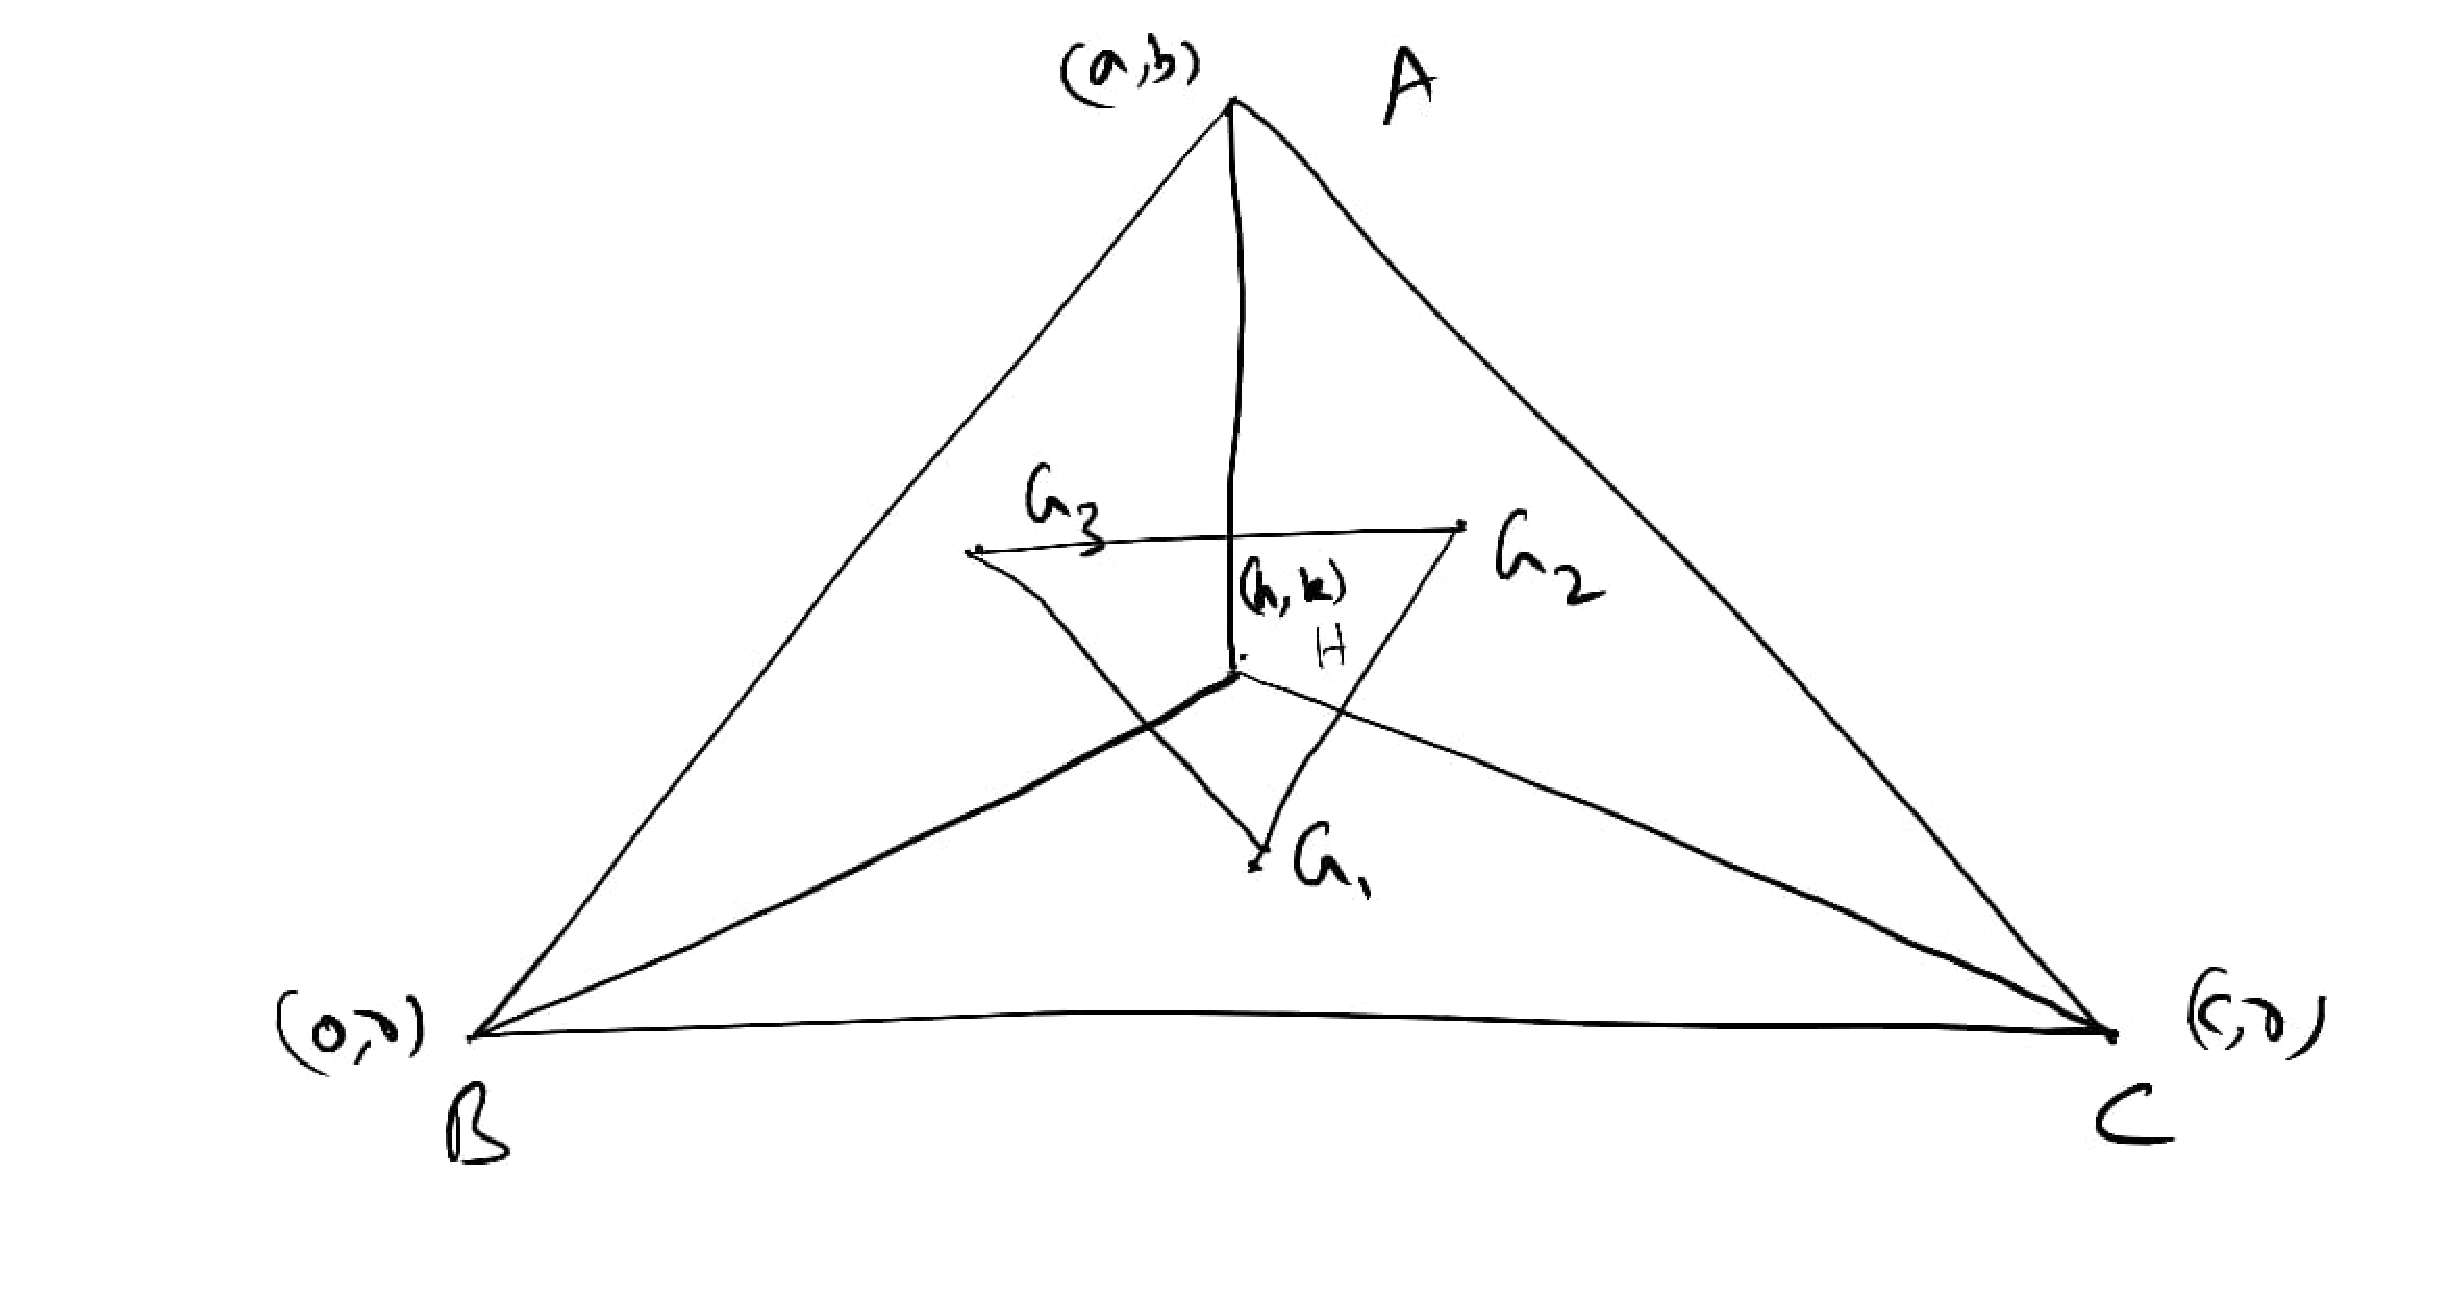
\includegraphics[width=\columnwidth]{./figs/prmo_2018_21.eps}
\caption{}
\label{fig:prmo_2018_21}
\end{figure}
%
\item A positive integer $k$ is said to be good if there exists a partition of $\cbrak{1, 2, 3,\dots, 20}$ in to disjoint proper subsets such that the sum of the numbers in each subset of the partition is $k$. How many good numbers are there? 
\item What is the largest positive integer $n$ such that 
\begin{align}
\frac{a^2}{\frac{b}{29}  + \frac{c}{ 31}} +
\frac{b^2}{ \frac{ c}{ 29} + \frac{a}{31}} +
\frac{c^2}{ \frac{a}{29}+ \frac{b}{ 31}} \ge n\brak{a+b+c}
\end{align}
holds for all positive real numbers a, b, c. 
\item  If N is the number of triangles of different shapes (i.e., not similar) whose angles are all integers (in degrees), what is N/100? 
\item  Let T be the smallest positive integer which, when divided by 11, 13, 15 leaves remainders in the sets {7, 8, 9}, {1, 2, 3}, {4, 5, 6} respectively. What is the sum of the squares of the digits of T? 
\item  What is the number of ways in which one can choose 60 unit squares from a $11 \times 11$ chessboard such that no two chosen squares have a side in common?
\item What is the number of ways in which one can colour the squares of a $4\times 4$ chessboard with colours red and blue such that each row as well as each column has exactly two red squares and two blue squares? 
\item Let N be the number of ways of distributing 8 chocolates of different brands among 3 children such that each child gets at least one chocolate, and no two children get the same number of chocolates. Find the sum of the digits of N.
\\
\solution The distribution of chocolates among the 3 children is illustrated by the Table \ref{table:prmo_2018_28}
\begin{table}[!ht]
\centering
\input{./figs/prmo_2018_28}
\caption{}
\label{table:prmo_2018_28}
\end{table}
%
Thus, the number of possible ways to distribute is 
\begin{multline}
\nCr{8}{1}\times
\nCr{7}{2}\times
\nCr{6}{5}
+
\nCr{8}{1}\times
\nCr{7}{3}\times
\nCr{6}{4} 
\\
= 8\times 21\times6+8\times35\times15 = 5208 
\end{multline}
%
Sum of the digits is 15.
\item Let $D$ be an interior point of the side $BC$ of a triangle $ABC$. Let $I_1$ and $I_2$ be the incentres of triangles $ABD$ and $ACD$ respectively. Let $AI_1$ and $AI_2$ meet $BC$ in $E$ and $F$ respectively. If $\angle BI_1E = 60 \degree$,, what is the measure of $\angle CI_2F$ in degrees?
\\
\solution In Fig. $\ref{fig:prmo_2018_29}$, we need to find $\theta$.  
\begin{enumerate}
\item $CI_2$ bisects $C$,  
\item $\theta$ is exterior to $\triangle AI_1 C$
\item $AI_2$ bisects $A$
\item $\angle ADB$ is exterior to $\triangle ADC$.
\end{enumerate}
Hence,
\begin{align}
\angle CAI_2 = \theta -\frac{C}{2} = \angle DAI_2,
\\
\angle ADB = 2\brak{\theta -\frac{C}{2}} + C = 2\theta
\end{align}
%
Using a similar approach, 
\begin{align}
\angle ADC = 2\times 60 \degree = 120 \degree
\end{align}
Thus, 
\begin{align}
2\theta + 120 \degree = 180 \degree \implies \theta = 30 \degree.
\end{align}
\begin{figure}[!ht]
\centering
\includegraphics[width=\columnwidth]{./figs/prmo_2018_29.eps}
\caption{}
\label{fig:prmo_2018_29}
\end{figure}
\item Let $P(x)= a_0 + a_1x+ a_2x^2 + \dots + a_nx^n$ be a polynomial in which $a_i$ is a non-negative integer for each $i \in \cbrak{0, 1, 2, 3, \dots ,n}$. If $P(1) = 4$ and $P(5) = 136$, what is the value of $P(3)$?

\end{enumerate}
\end{document}


